\documentclass[11pt,a4paper]{article}
\usepackage[margin=0.76in]{geometry}
\usepackage[T1]{fontenc}
\usepackage{lmodern}
\usepackage{amsmath,amssymb}
\usepackage{graphicx}
\usepackage{float}
\usepackage{microtype}
\usepackage[hidelinks]{hyperref}
\emergencystretch=3em

\newcommand{\G}{\mathcal G}
\newcommand{\B}{\mathbb B}

\title{Greedy Classes Need Not Be Linear\\[0.3em]
\large The question in arXiv:1303.4972 was answered by arXiv:0911.4900}
\author{Automated Mathematics Run \texttt{fa\_banach\_001}, lane 0}
\date{13 August 2026}

\begin{document}
\sloppy
\hbadness=2000
\maketitle

\begin{center}
\fbox{\parbox{0.92\linewidth}{\textbf{Status: literature already answered
(negative).} No new theorem is claimed.  The literal universal question has
an explicit counterexample in the cited earlier paper of Garrig\'os,
Hern\'andez, and de Natividade.  Choosing its exponents $p=2$ and $r=1$
keeps the example inside the Banach-space and lattice-unconditional setting
of arXiv:1303.4972.}}
\end{center}

\section{The source question}

For a normalized basis $(e_n)$ in a Banach space, let $\gamma_N(x)$ be the
largest error among thresholding greedy approximants of order $N$ (the
maximum only matters when coefficients tie).  Wojtaszczyk defines the greedy
classes by replacing the best $N$-term error in the usual approximation-space
quasi-norm by $\gamma_N(x)$.  For the endpoint parameter,
\[
 \G_\infty^\alpha
 =\left\{x:\ \|x\|+\sup_{N\ge1}N^\alpha\gamma_N(x)<\infty\right\}.
\]
The paper then says that it is not known whether $\G_q^\alpha$ is a linear
space.  Read as the natural universal question over the paper's fixed but
otherwise arbitrary unconditional basis, the answer is no.

\begin{figure}[H]
  \centering
  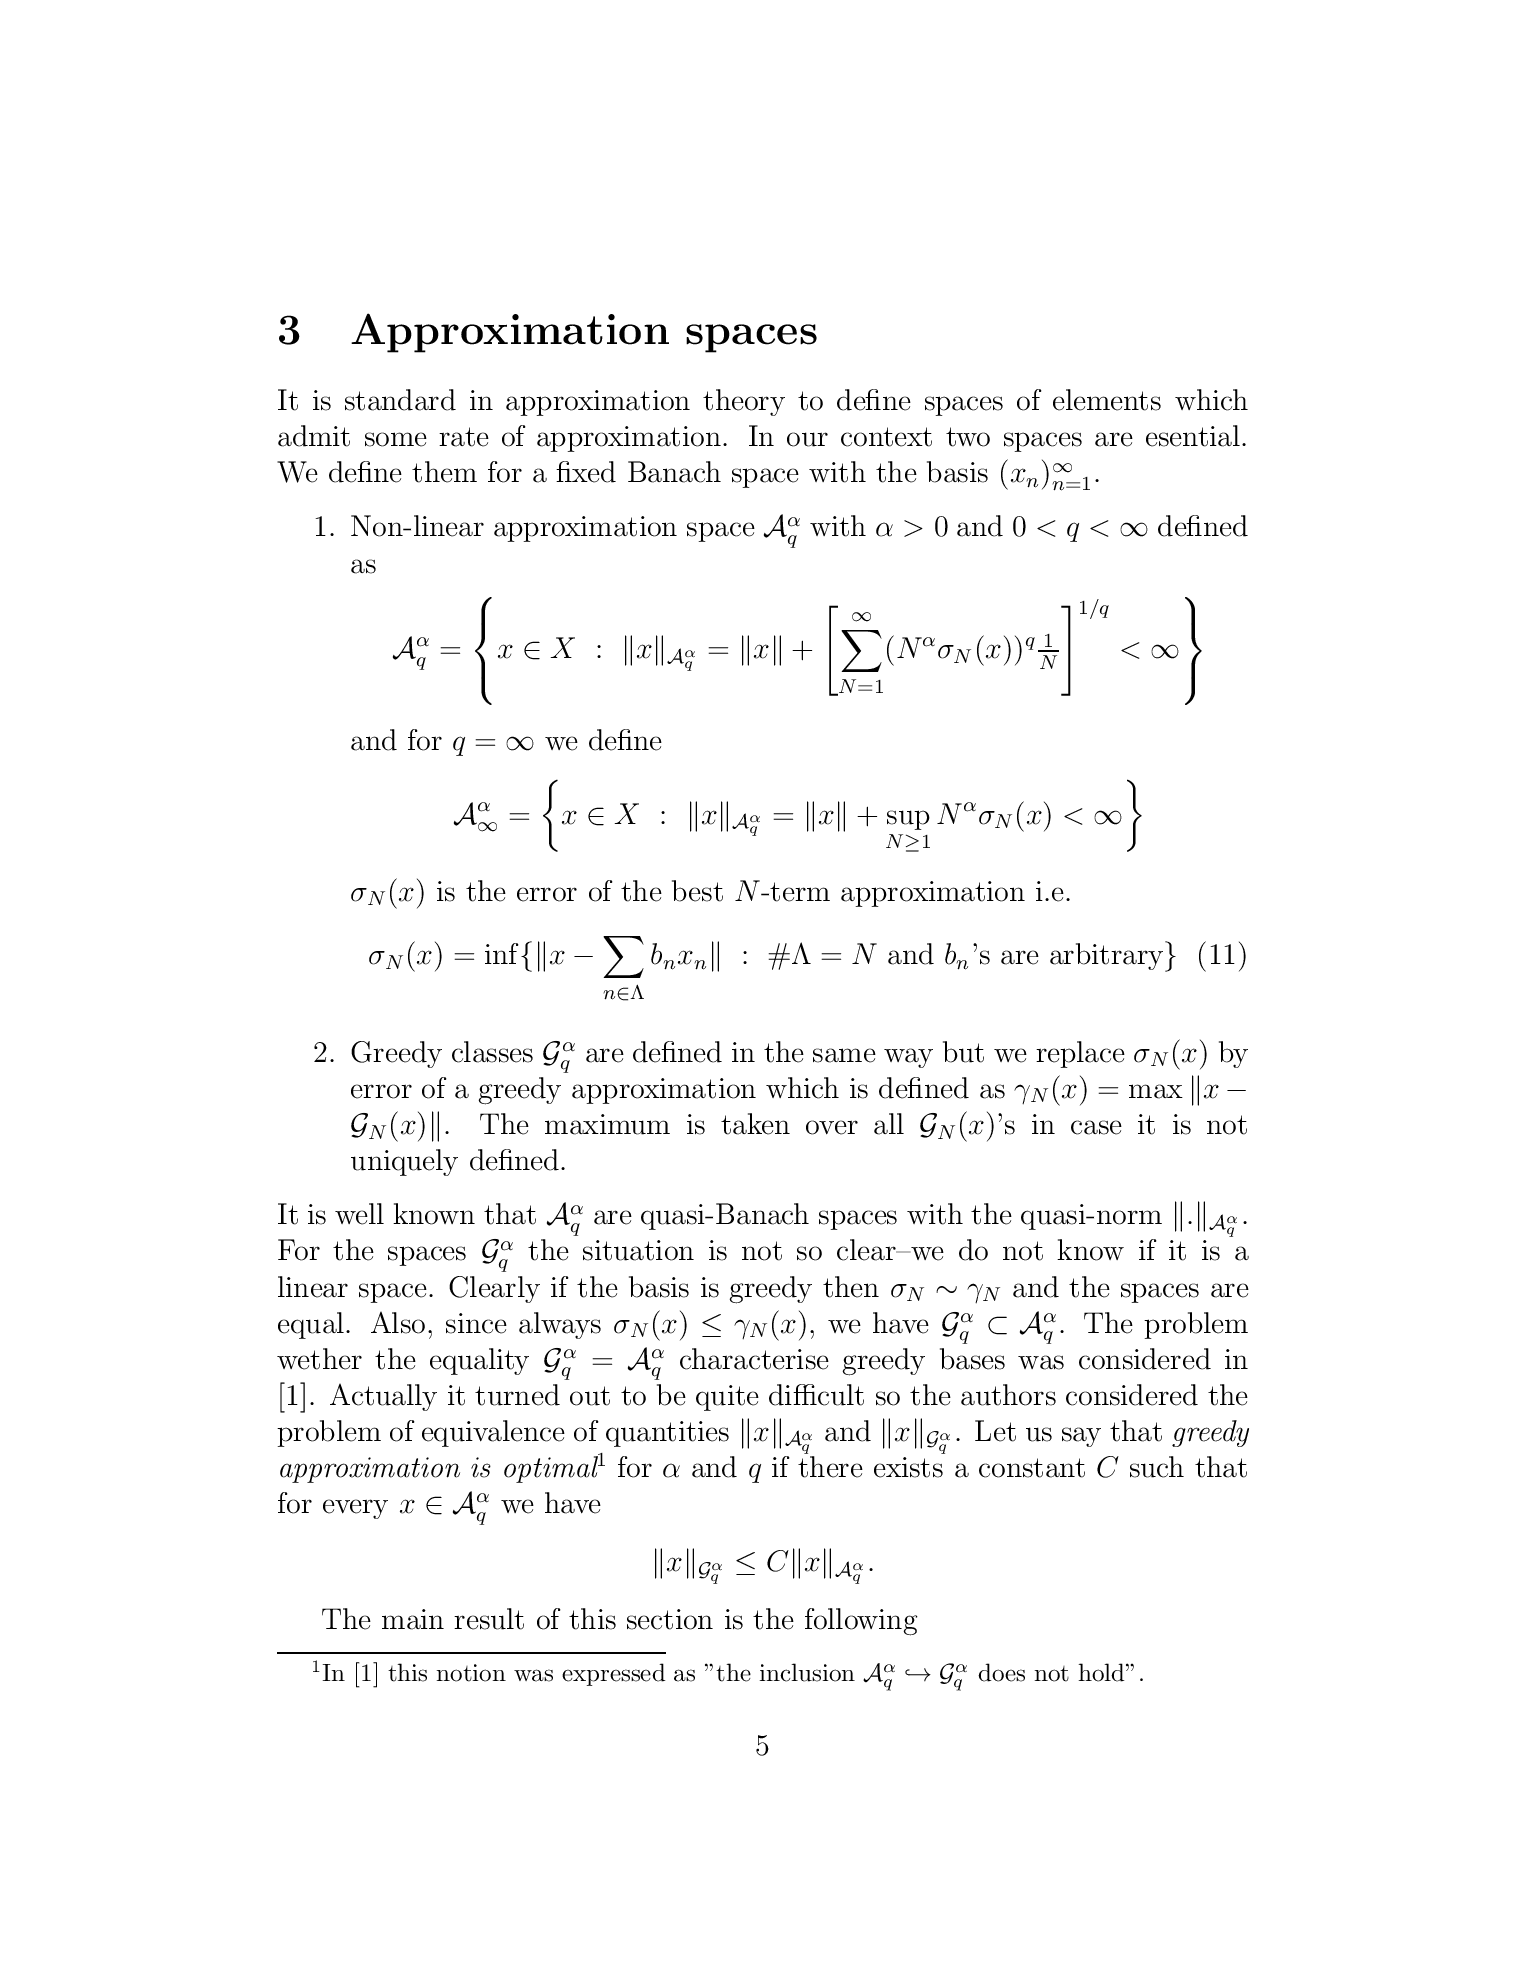
\includegraphics[width=0.82\linewidth,trim=0 212 0 332,clip]{figures/source_question_page_5.png}
  \caption{Wojtaszczyk, arXiv:1303.4972, PDF page 5.}
\end{figure}

\clearpage
\section{The earlier counterexample}

Section 7.2 of Garrig\'os--Hern\'andez--de Natividade (arXiv:0911.4900,
published in 2012) takes
\[
 \B=\ell^p\oplus_{\ell^1}\ell^r,
 \qquad 0<r<p<\infty,
\]
with its canonical basis.  To match the later paper's hypotheses, take for
example $p=2$ and $r=1$.  Then $\B$ is a Banach space and the canonical basis
is normalized and lattice unconditional.

Fix $\alpha>0$, put
\[
 \beta=\alpha+\frac1p,\qquad
 \gamma=\alpha+\frac1r,
\]
and define
\[
 x=((k^{-\beta})_{k\ge1},0),\qquad
 y=(0,(j^{-\gamma})_{j\ge1}).
\]
Since $\beta p=\alpha p+1$ and $\gamma r=\alpha r+1$, integral
comparison gives
\[
 \gamma_N(x)=\left(\sum_{k>N}k^{-\beta p}\right)^{1/p}
 \asymp N^{-\alpha},\qquad
 \gamma_N(y)=\left(\sum_{j>N}j^{-\gamma r}\right)^{1/r}
 \asymp N^{-\alpha}.
\]
Consequently $x,y\in\G_\infty^\alpha$.

\begin{figure}[H]
  \centering
  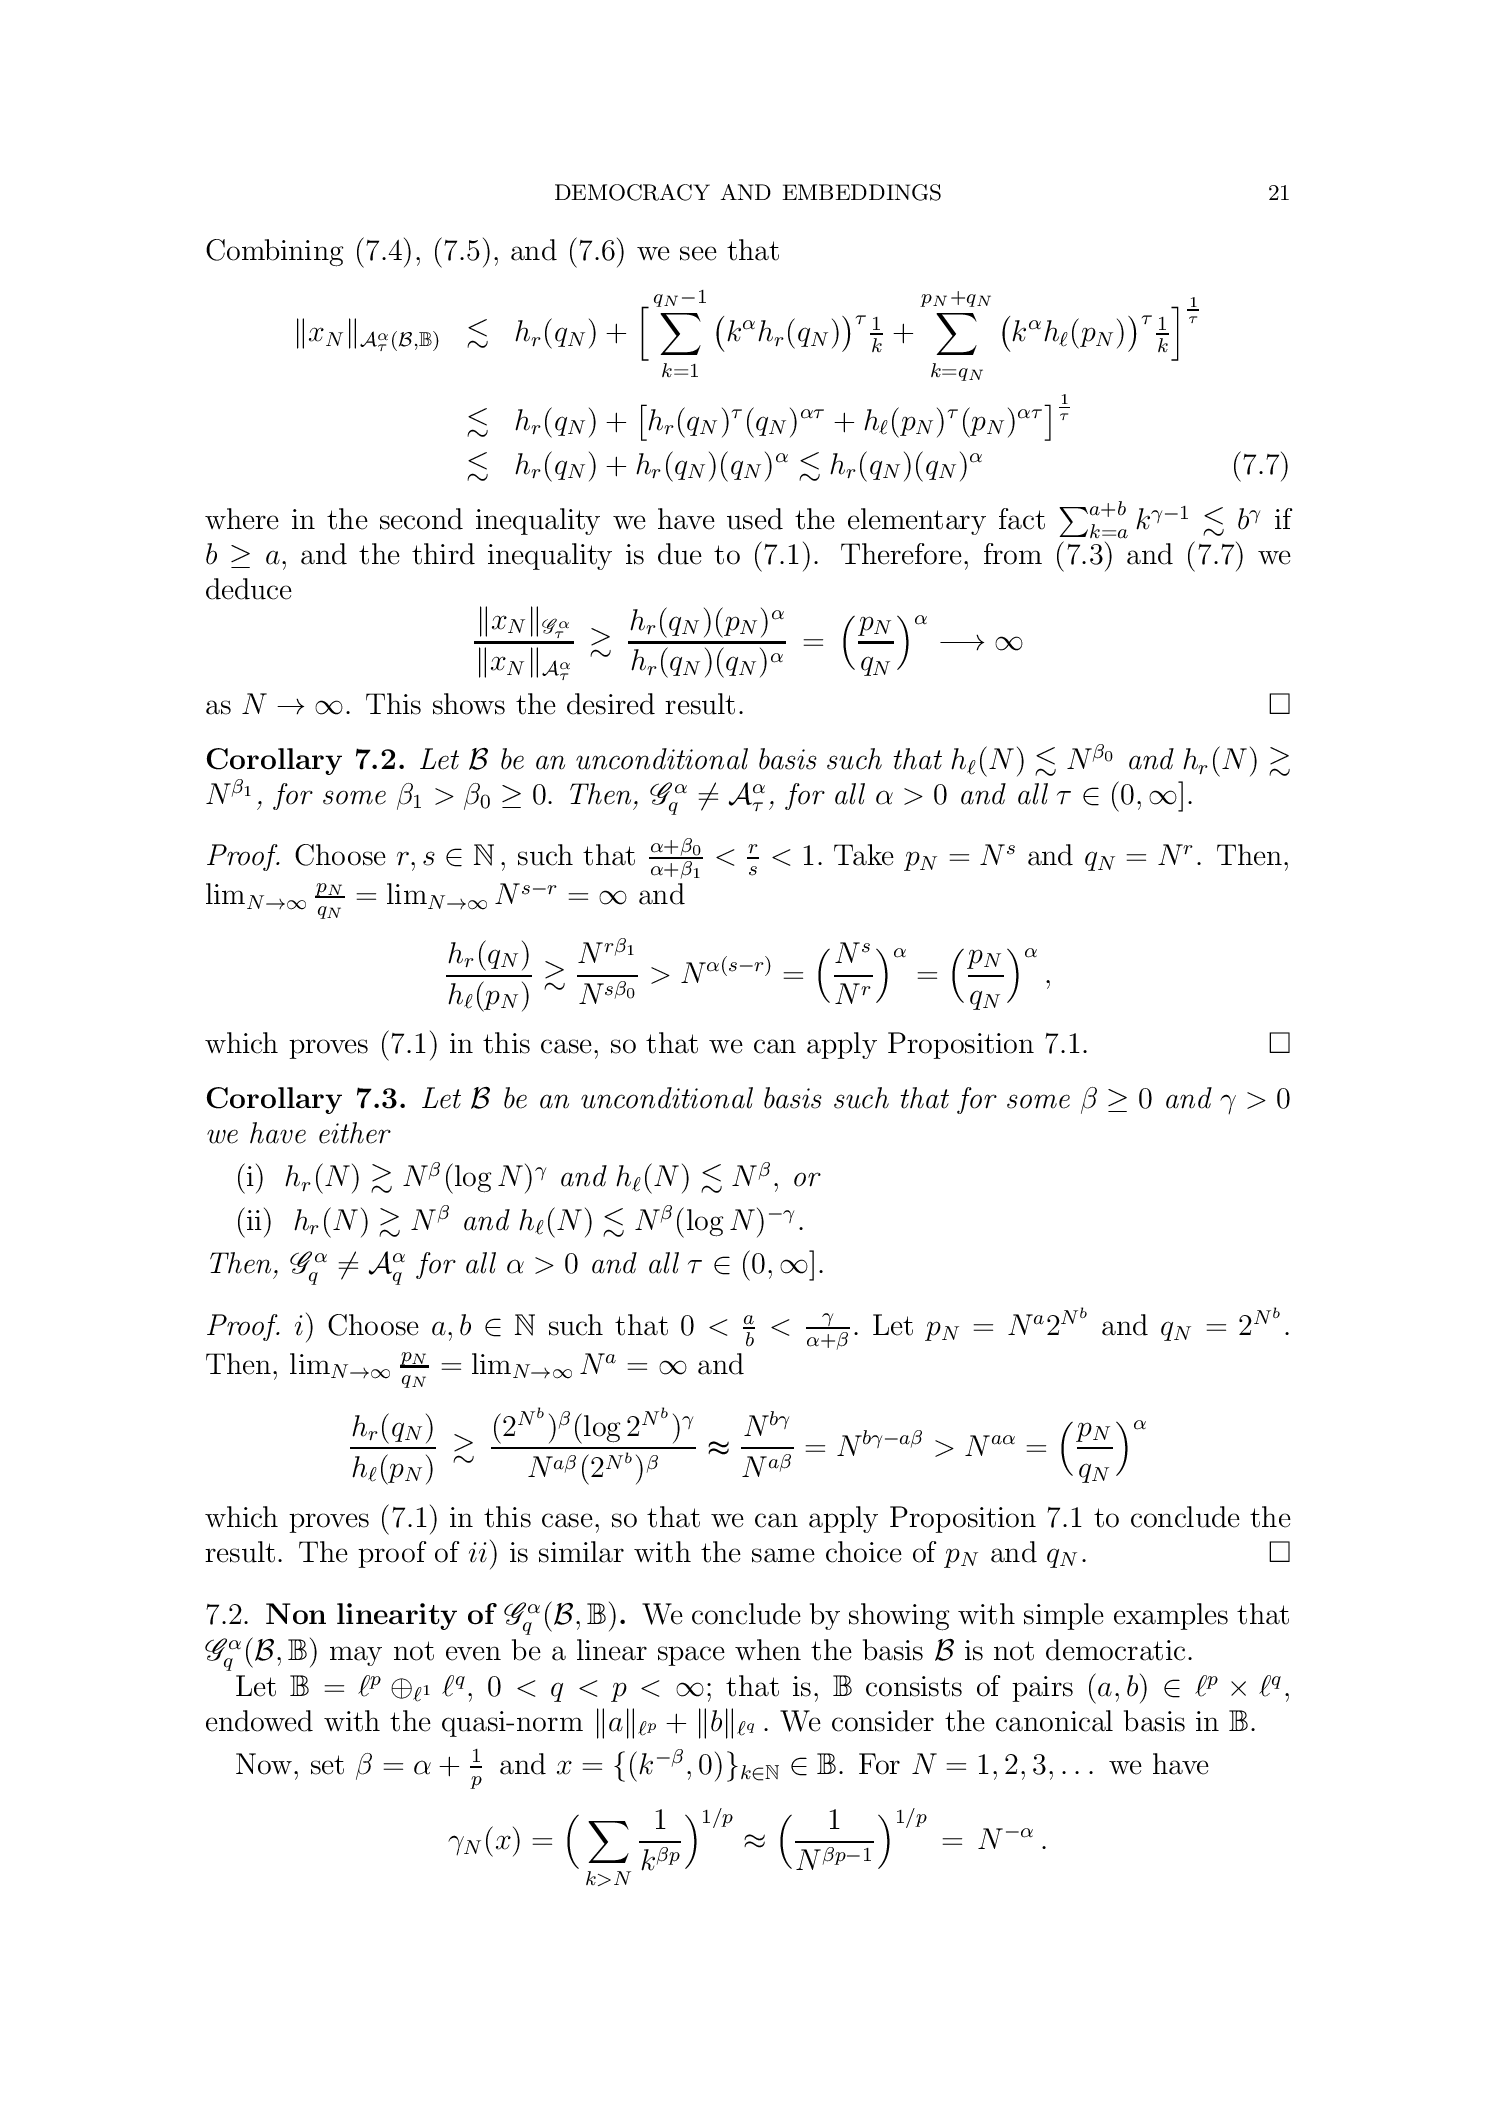
\includegraphics[width=0.86\linewidth,trim=0 0 0 572,clip]{figures/supporting_setup_page_21.png}
  \caption{Earlier paper, PDF page 21: start of Section 7.2.}
\end{figure}

\clearpage
\section{Why the sum leaves the class}

Here $r<p$, hence $\gamma>\beta$.  Group the $x$-coefficients whose sizes
lie between two consecutive $y$-coefficients:
\[
 A_j=\{k:\ j^{-\gamma}\le k^{-\beta}<(j-1)^{-\gamma}\}.
\]
Then $|A_j|\asymp j^{\gamma/\beta-1}$.  At the greedy orders
\[
 N_J=J+\sum_{j=1}^J|A_j|\asymp J^{\gamma/\beta},
\]
the retained coefficients are, up to harmless boundary ties, precisely the
first $J$ coefficients of $y$ together with the $x$-coefficients in the first
$J$ blocks.  Therefore
\begin{align*}
 \gamma_{N_J}(x+y)
 &\asymp
 \left(\sum_{k>J^{\gamma/\beta}}k^{-\beta p}\right)^{1/p}
 +\left(\sum_{j>J}j^{-\gamma r}\right)^{1/r}\\
 &\asymp J^{-\alpha\gamma/\beta}+J^{-\alpha}
 \asymp J^{-\alpha}
 \asymp N_J^{-\alpha\beta/\gamma}.
\end{align*}
It follows that
\[
 N_J^\alpha\gamma_{N_J}(x+y)
 \asymp N_J^{\alpha(1-\beta/\gamma)}\longrightarrow\infty,
\]
so $x+y\notin\G_\infty^\alpha$.  Thus $\G_\infty^\alpha$ is not a
linear space, for every $\alpha>0$, even for a normalized
lattice-unconditional basis of a Banach space.  This settles the literal
universal question negatively.  The earlier paper also states that a simple
modification treats every finite class parameter, but that stronger assertion
is not needed for the negative answer recorded here.

\begin{figure}[H]
  \centering
  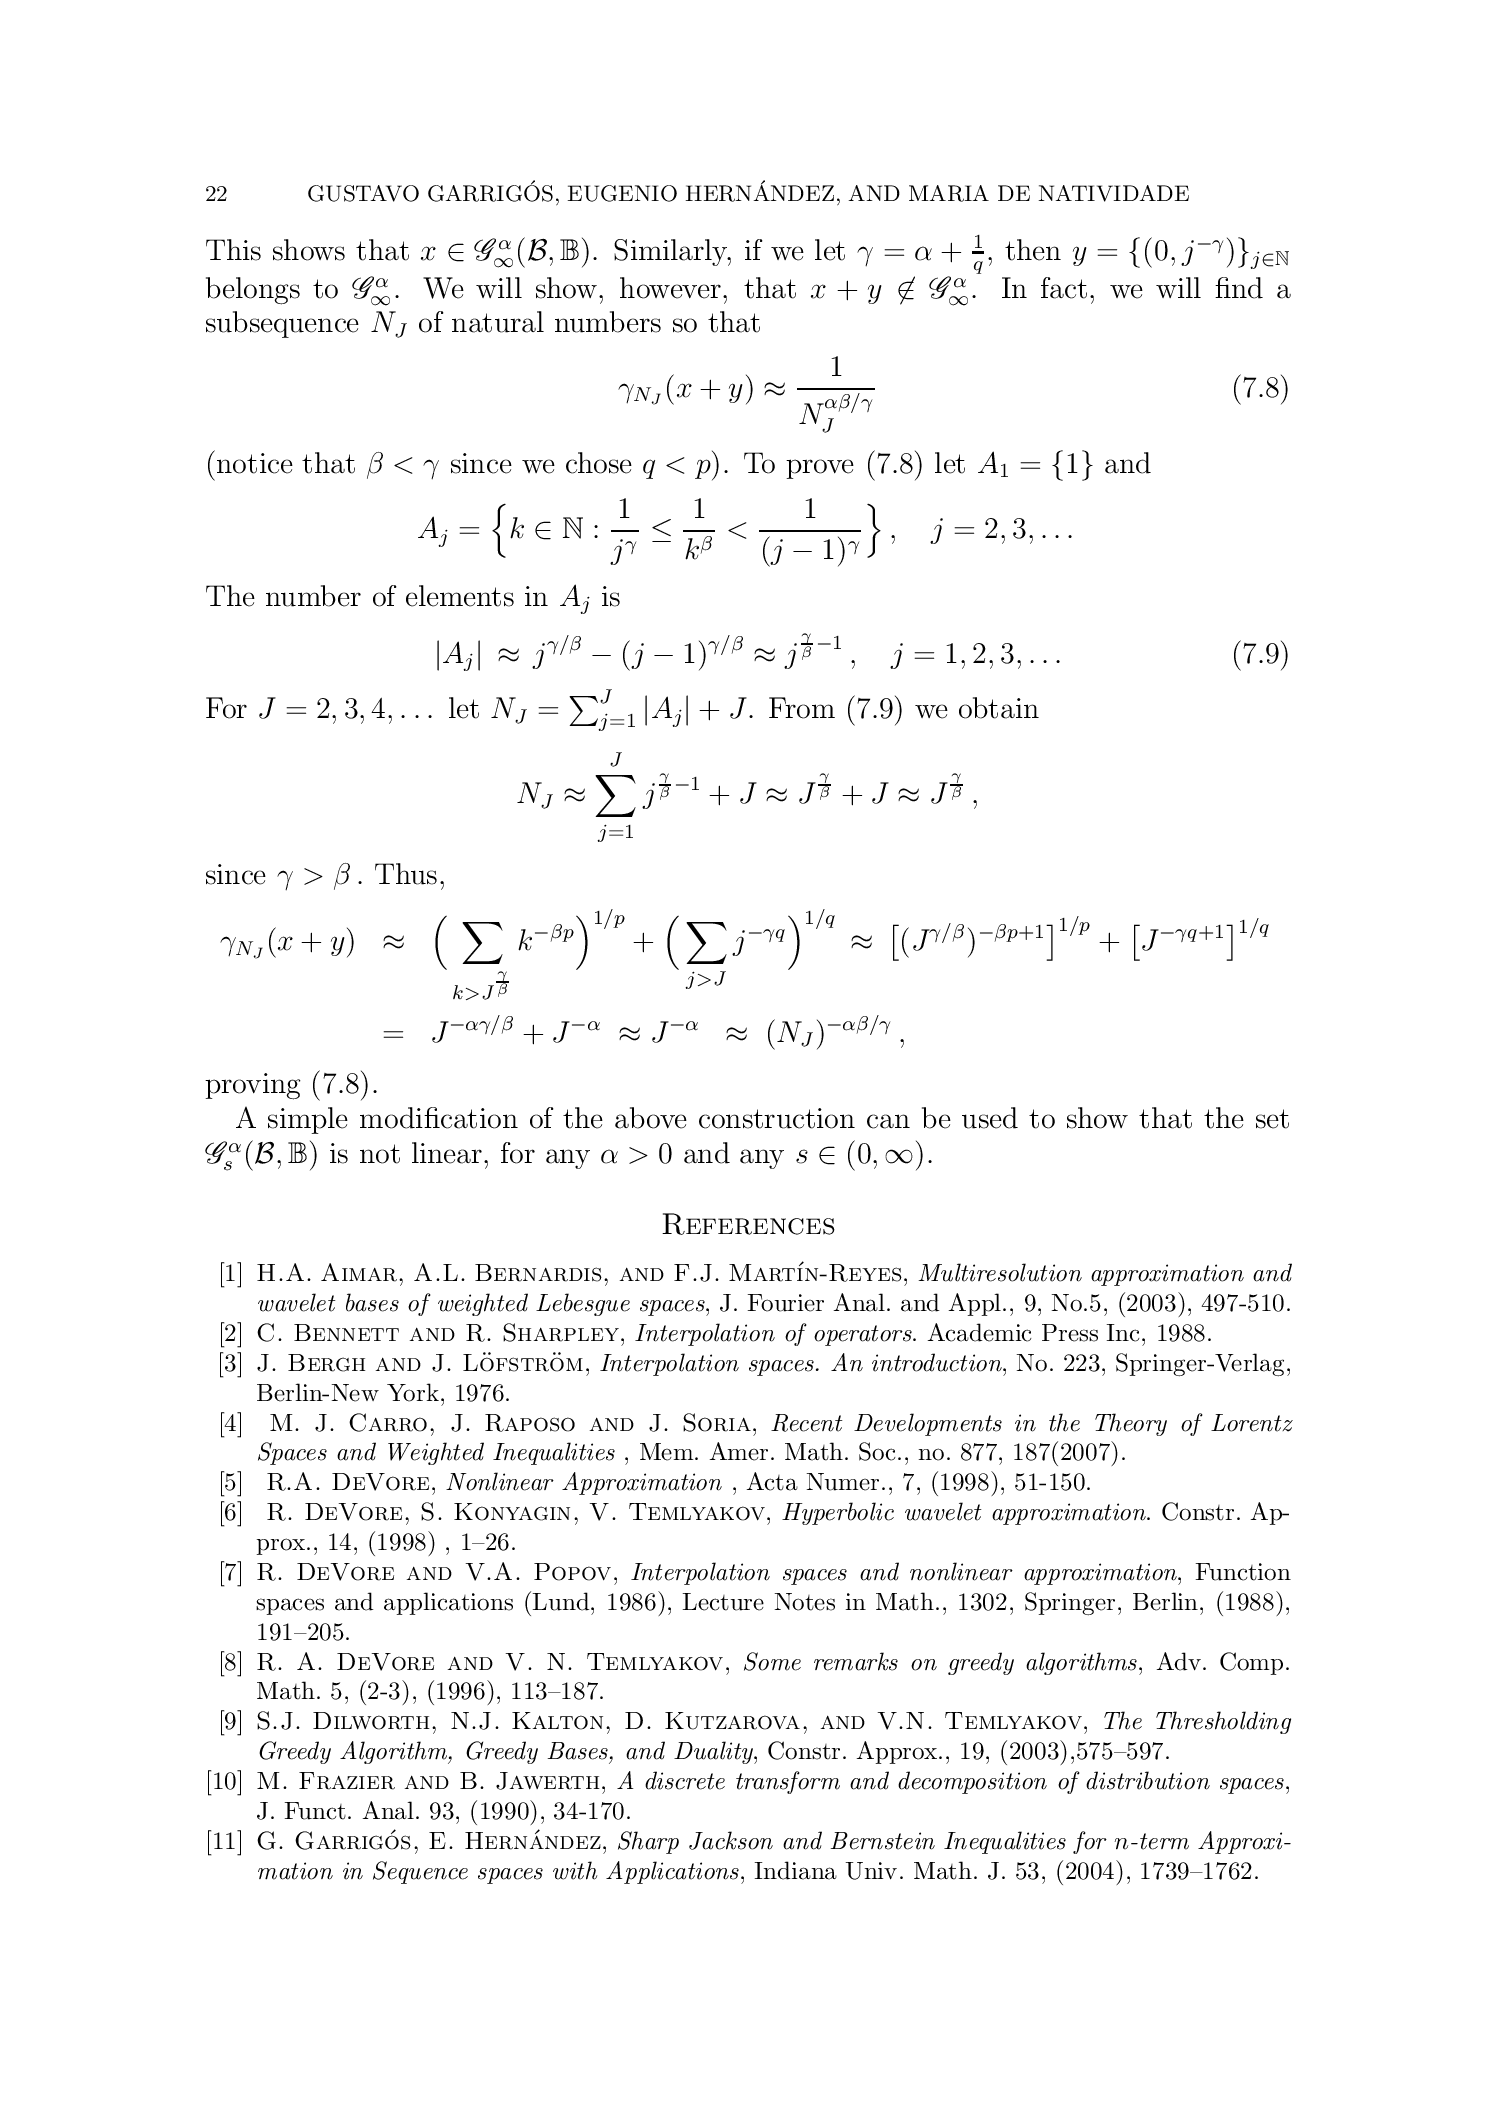
\includegraphics[width=0.72\linewidth,trim=0 422 0 40,clip]{figures/supporting_conclusion_page_22.png}
  \caption{Earlier paper, PDF page 22: the rate computation and conclusion.}
\end{figure}

\section{Provenance and scope}

The question was checked directly on page 5 of arXiv:1303.4972.  The complete
counterexample was checked on pages 21--22 of arXiv:0911.4900.  The latter is
G.~Garrig\'os, E.~Hern\'andez, and M.~de Natividade,
\emph{Democracy functions and optimal embeddings for approximation spaces},
Advances in Computational Mathematics 37 (2012), 255--283,
DOI \href{https://doi.org/10.1007/s10444-011-9197-0}{10.1007/s10444-011-9197-0}.
It is cited as reference [1] by arXiv:1303.4972.  This packet records an
earlier-literature disposition only; it makes no novelty claim.  If the
source sentence was intended to ask about one particular basis constructed
elsewhere in that paper rather than the general class just defined, the
earlier example does not decide that narrower, unstated question.

\end{document}
